% AMSC-HAR project report
% Compile: pdflatex main.tex && pdflatex main.tex
\documentclass[11pt,a4paper]{article}

\usepackage[T1]{fontenc}
\usepackage[utf8]{inputenc}
\usepackage{lmodern}
\usepackage[margin=2.2cm]{geometry}
\usepackage{amsmath,amssymb,amsthm}
\usepackage{booktabs}
\usepackage{graphicx}
\usepackage{tikz}
\usetikzlibrary{arrows.meta,positioning,fit,calc,chains}
\usepackage{xcolor}
\usepackage{listings}
\usepackage{hyperref}
\usepackage{enumitem}
\usepackage{caption}
\usepackage{setspace}
\usepackage{titlesec}

\hypersetup{
  colorlinks=true,
  linkcolor=black,
  citecolor=black,
  urlcolor=blue!50!black
}

\definecolor{codebg}{RGB}{247,247,248}
\lstset{
  basicstyle=\ttfamily\footnotesize,
  backgroundcolor=\color{codebg},
  frame=single,
  framerule=0.3pt,
  rulecolor=\color{black!20},
  breaklines=true,
  columns=fullflexible,
  keepspaces=true,
  xleftmargin=0.4em,
  xrightmargin=0.4em,
  aboveskip=0.7em,
  belowskip=0.7em
}

\titleformat{\section}{\large\bfseries}{\thesection}{0.6em}{}
\titleformat{\subsection}{\normalsize\bfseries}{\thesubsection}{0.5em}{}
\setlist[itemize]{leftmargin=1.4em,itemsep=0.15em,topsep=0.25em}
\setlist[enumerate]{leftmargin=1.4em,itemsep=0.15em,topsep=0.25em}
\setlength{\parskip}{0.35em}
\setlength{\parindent}{0pt}
\onehalfspacing

\title{\textbf{Video Based Human Action Recognition}}
\author{AMSC-HAR\\
Politecnico di Milano\\
Advanced Methods for Scientific Computing}
\date{\today}

\begin{document}
\maketitle
\vspace{-1.2em}

\begin{abstract}
This report describes \textbf{AMSC-HAR}, a header-only C++23 library and
command-line trainer for video-based human action recognition.
Unlike typical student projects that wrap PyTorch or TensorFlow, the system
implements tensors, layers, automatic-style reverse-mode gradients, SGD,
checkpointing, video decoding, and optional CUDA kernels from scratch.
The model is a compact VideoCNN: a shared 2D convolutional backbone over
sampled RGB frames, a residual temporal 1D convolution, learnable temporal
attention pooling, and a linear classifier.
On the UCF11 (YouTube Action) dataset the default recipe uses $64\times 64$
frames, $T=8$ uniformly sampled time steps, and about $5.9\times 10^5$
trainable parameters.
A held-out inference check with the released best checkpoint
\texttt{ucf11\_videocnnBest.harw} classified $8/10$ randomly drawn clips
correctly (80\%), with several classes predicted at $>95\%$ confidence.
The same codebase also targets UCF101 official splits.
This document covers design goals, software architecture, the mathematical
model, the data pipeline, training, the CUDA backend, and experimental
results.
\end{abstract}

\tableofcontents
\vspace{0.6em}

%----------------------------------------------------------------------
\section{Introduction}
\label{sec:intro}

Human action recognition (HAR) from video represents a significant area of research within the domain of computer vision, addressing challenges such as real-world variability, computational efficiency, and robust feature extraction~\cite{houssein2025integrating}. Recent literature highlights the synergistic combination of Soft Computing (SC) paradigms---such as Neural Networks---and Multi-Agent Systems (MAS) as a robust strategy to overcome these challenges~\cite{houssein2025integrating}. A short clip must be mapped to one of a fixed set of action classes (e.g.\ \emph{diving}, \emph{tennis swing}, \emph{walking a dog}). The academic community usually solves this with large 3D CNNs or transformer video models trained in Python frameworks.
Those stacks hide the linear algebra, memory layout, and gradient bookkeeping
that a scientific-computing course is meant to expose.

Following the directions outlined by Houssein et al.~\cite{houssein2025integrating} for efficient and robust HAR systems, AMSC-HAR takes the opposite route to traditional frameworks. The project represents a foundational Soft Computing component (a from-scratch Neural Network) capable of being integrated into larger distributed Multi-Agent frameworks, providing a \emph{complete} recognition pipeline written in modern C++:
\begin{itemize}
  \item a generic \texttt{Tensor<T>} with CPU storage and optional
        CUDA Unified Memory;
  \item layers with explicit \texttt{forward}/\texttt{backward} (Conv2D,
        BatchNorm2D, ReLU, pooling, Dropout, Linear, TemporalConv1D,
        temporal attention);
  \item SGD with momentum and $\ell_2$ weight decay;
  \item softmax cross-entropy;
  \item OpenCV (or FFmpeg) video decoding, a binary clip cache, and
        train-time augmentation;
  \item a custom checkpoint format \texttt{.harw};
  \item a single executable \texttt{har\_cnn} for smoke tests, training,
        prediction, and split evaluation.
\end{itemize}

\paragraph{Contributions.}
(1)~A compact, auditable VideoCNN that stays under 0.6M parameters while
remaining strong on UCF11.
(2)~A dual CPU/CUDA path so the same headers train on a laptop or a GPU.
(3)~An end-to-end data path (decode $\to$ cache $\to$ temporal sample
$\to$ batch) that makes repeated epochs practical.
(4)~Reproducible CLI defaults (seed 42, $80/10/10$ UCF11 split) and a
self-describing weight file that stores image size, clip length, and class
names.

\paragraph{Report outline.}
Section~\ref{sec:bg} recalls HAR and the datasets.
Section~\ref{sec:tensor} describes tensors and layers.
Section~\ref{sec:model} specifies VideoCNN.
Section~\ref{sec:data} covers decoding and augmentation.
Section~\ref{sec:exp} reports experiments.
Section~\ref{sec:conc} concludes.

%----------------------------------------------------------------------
\section{Background and problem statement}
\label{sec:bg}

\subsection{Video action recognition}

Action recognition represents a vital domain within computer vision, utilizing various data types to analyze human activities~\cite{houssein2025integrating}. A video is a tensor $X\in\mathbb{R}^{T\times C\times H\times W}$. The classifier produces logits $z\in\mathbb{R}^{K}$ and a predicted class $\hat{y}=\arg\max_k z_k$. As highlighted by recent studies~\cite{houssein2025integrating}, traditional methods are being replaced by Deep Learning and Soft Computing techniques capable of automatically extracting spatio-temporal features. While recent work uses 3D CNNs and space--time transformers which are accurate but computationally expensive, efficient models are required for real-time deployment and distributed sensing environments.

AMSC-HAR uses a cheaper and more transparent design:
\emph{2D CNN on each frame}, then a \emph{1D temporal mixer} and
\emph{attention pooling}.
This late temporal aggregation provides a transparent Soft Computing design where the temporal conv and attention are trained jointly with the backbone, ensuring computational efficiency~\cite{houssein2025integrating}.

\subsection{Datasets}

\paragraph{UCF11} (YouTube Action) contains 11 sport and
daily actions, originally published as MPEG clips crawled from YouTube.
This project uses the updated \texttt{UCF11\_updated\_mpg} release
(1600 clips after scanning the extracted tree).
UCF11 has no official train/test list, so the loader applies a
class-stratified shuffle with default ratios
$80\%$ train / $10\%$ val / $10\%$ test.

\paragraph{UCF101} has 101 classes and three official
recognition splits.
This dataset is used to evaluate the performance of the VideoCNN model.

Table~\ref{tab:ucf11} lists the UCF11 classes as stored in the best
checkpoint (alphabetical folder names).

\begin{table}[htbp]
\centering
\caption{UCF11 classes and clip counts in \texttt{data/UCF11\_updated\_mpg}.}
\label{tab:ucf11}
\small
\begin{tabular}{@{}lrlr@{}}
\toprule
\textbf{Class} & \textbf{Clips} & \textbf{Class} & \textbf{Clips} \\
\midrule
basketball            & 141 & soccer\_juggling      & 156 \\
biking                & 145 & swing                 & 137 \\
diving                & 156 & tennis\_swing         & 167 \\
golf\_swing           & 142 & trampoline\_jumping   & 119 \\
horse\_riding         & 198 & volleyball\_spiking   & 116 \\
                      &     & walking               & 123 \\
\midrule
\multicolumn{3}{@{}l}{Total} & 1600 \\
\bottomrule
\end{tabular}
\end{table}

\section{Tensor library and layers}
\label{sec:tensor}

\subsection{Tensors}

\texttt{har::Tensor<T>} is a dense, row-major, contiguous array with an
explicit shape and computed strides.
Images and activations use NCHW layout, which matches both the CPU
convolution loops and the CUDA kernels.
Allocation is either \texttt{new T[n]} on the host or
\texttt{cudaMallocManaged} when the default device is CUDA.
Elementwise arithmetic, \texttt{reshape}/\texttt{reshaped}, and
\texttt{sync()} (a device-wide barrier when CUDA is active) are provided
in the header.

A \texttt{Parameter<T>} pairs a data tensor with a same-shaped gradient
and a \texttt{requires\_grad} flag.
SGD and checkpointing iterate parameter lists; BatchNorm additionally
exposes non-parameter running mean/variance in the state dict.

\subsection{Layer contract}

Every spatial layer implements
\begin{align*}
  y &= f(x;\theta), &
  g_x &= \frac{\partial L}{\partial x}
       = \Bigl(\frac{\partial y}{\partial x}\Bigr)^{\!\!\top} g_y,
\end{align*}
by caching $x$ (and any auxiliaries) during \texttt{forward} and using
them in \texttt{backward}.
There is no tape interpreter: the graph is the C++ call stack of
\texttt{VideoCNN::forward} / \texttt{backward}.
This is easy to debug and maps one-to-one onto the kernels in
\texttt{cuda\_ops.cu}.

\subsection{Spatial operators}

\paragraph{Conv2D.}
A $K_h\times K_w$ kernel with stride $(s_h,s_w)$ and padding $(p_h,p_w)$
implements
\[
  y_{n,c',h',w'}
  = b_{c'} + \sum_{c,i,j} W_{c',c,i,j}\,
    x_{n,c,\,s_h h'+i-p_h,\,s_w w'+j-p_w}.
\]
Weights use a simple scaled-uniform init.
The CPU path is a direct 7-loop implementation; the CUDA path launches
\texttt{conv2d\_forward}/\texttt{conv2d\_backward}.

\paragraph{BatchNorm2D.}
Channel statistics are computed over $N\cdot H\cdot W$.
In training,
\[
  \hat x_c = \frac{x_c-\mu_c}{\sqrt{\sigma_c^2+\varepsilon}},\qquad
  y_c = \gamma_c\hat x_c + \beta_c,
\]
and $(\mu,\sigma^2)$ are written into exponential moving averages
(momentum $0.1$).
Eval uses the running statistics stored in the checkpoint, which is
essential for the 80\% folder test in Section~\ref{sec:exp}.

\paragraph{Pooling and activations.}
$2\times 2$ max-pool records argmax indices for the backward pass.
Global average pool collapses $H\times W$ to a 256-D frame embedding.
ReLU is $y=\max(x,0)$.
Dropout ($p=0.3$) is applied only on the pooled vector, and only in
training.

\paragraph{Linear and loss.}
The head is $z = W h + b$ with $W\in\mathbb{R}^{K\times 256}$.
Cross-entropy is the stable softmax + NLL
\[
  \ell = -\frac{1}{N}\sum_{n=1}^{N}\log
  \frac{e^{z_{n,y_n}-\max_k z_{n,k}}}
       {\sum_{j} e^{z_{n,j}-\max_k z_{n,k}}}.
\]
The backward gradient is $(\mathrm{softmax}(z)-e_y)/N$, moved back to the
activation device.

\subsection{Optimiser}

SGD with momentum $m=0.9$ and weight decay $\lambda=10^{-4}$ updates
\[
  v \leftarrow m v + (g + \lambda \theta),\qquad
  \theta \leftarrow \theta - \eta v.
\]
The learning rate starts at $\eta=3\cdot 10^{-3}$ and is multiplied by
$\gamma=0.5$ every 4 epochs (\texttt{--lr-step}).
Velocity buffers are allocated lazily to match parameter shapes and
devices.

%----------------------------------------------------------------------
\section{VideoCNN architecture}
\label{sec:model}

\subsection{Forward pass}

Let a batch of clips be $X\in\mathbb{R}^{N\times T\times 3\times H\times W}$
with default $H=W=64$ and $T=8$.
Time is flattened to a 2D batch of $NT$ frames.
A four-stage backbone produces a 256-D vector per frame; a temporal
residual block mixes neighbouring frames; attention pools time; a linear
layer outputs $K$ logits (Figure~\ref{fig:cnn}).

\begin{figure}[t]
\centering
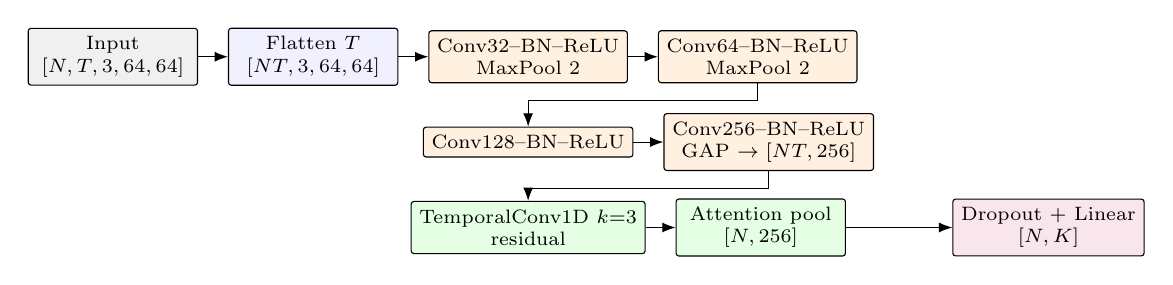
\begin{tikzpicture}[
  font=\scriptsize,
  node distance=0.38cm,
  blk/.style={draw, rounded corners=1pt, align=center, inner sep=3pt,
              minimum width=2.15cm, fill=blue!6},
  dim/.style={font=\tiny\ttfamily, text=black!55}
]
\node[blk, fill=gray!12] (in) {Input\\$[N,T,3,64,64]$};
\node[blk, right=of in] (flat) {Flatten $T$\\$[NT,3,64,64]$};
\node[blk, right=of flat, fill=orange!12] (c1) {Conv32--BN--ReLU\\MaxPool $2$};
\node[blk, right=of c1, fill=orange!12] (c2) {Conv64--BN--ReLU\\MaxPool $2$};
\node[blk, below=0.55cm of c1, fill=orange!12] (c3) {Conv128--BN--ReLU};
\node[blk, right=of c3, fill=orange!12] (c4) {Conv256--BN--ReLU\\GAP $\to[NT,256]$};
\node[blk, below=0.55cm of c3, fill=green!10] (tc) {TemporalConv1D $k{=}3$\\residual};
\node[blk, right=of tc, fill=green!10] (at) {Attention pool\\$[N,256]$};
\node[blk, right=1.35cm of at, fill=purple!10] (hd) {Dropout + Linear\\$[N,K]$};
\draw[-{Latex}] (in) -- (flat);
\draw[-{Latex}] (flat) -- (c1);
\draw[-{Latex}] (c1) -- (c2);
\draw[-{Latex}] (c2.south) -- ++(0,-0.22) -| (c3);
\draw[-{Latex}] (c3) -- (c4);
\draw[-{Latex}] (c4.south) -- ++(0,-0.22) -| (tc);
\draw[-{Latex}] (tc) -- (at);
\draw[-{Latex}] (at) -- (hd);
\end{tikzpicture}
\caption{VideoCNN data path. Spatial stages are shared across time; the
temporal block is residual ($h + \mathrm{TConv}(h)$).}
\label{fig:cnn}
\end{figure}

Spatial spatial sizes after padding-1 $3\times 3$ convolutions:
$64\!\to\!32$ (pool), $32\!\to\!16$ (pool), then $16\times 16$ until GAP.
Because image size must be divisible by 4, \texttt{build\_video\_cnn}
rejects illegal \texttt{--size} values.

\subsection{Temporal convolution and attention}

TemporalConv1D treats the $NT$ frame embeddings as $N$ sequences of length
$T$ and applies a depth-preserving 1D convolution of kernel size 3 with
zero-pad $1$:
\[
  u_{n,t,c'}
  = b_{c'} + \sum_{c=1}^{256}\sum_{k=-1}^{1}
    W_{c',c,k}\, h_{n,\,\mathrm{clamp}(t+k),\,c}.
\]
The residual $h+u$ lets the network keep a pure per-frame representation
when the temporal kernel is not yet useful.

Temporal attention pooling scores each time step with a learned query
$w\in\mathbb{R}^{256}$ (zero-initialised, so the first step equals a
temporal mean):
\begin{align}
  s_{n,t} &= h_{n,t}^{\top} w, &
  \alpha_{n,t} &= \frac{e^{s_{n,t}-\max_{t'}s_{n,t'}}}
                      {\sum_{t'} e^{s_{n,t'}-\max_{t''}s_{n,t''}}},
  \nonumber\\
  \bar h_n &= \sum_{t=1}^{T} \alpha_{n,t}\, h_{n,t}.
  \label{eq:attn}
\end{align}
The classifier then sees a single 256-D clip embedding.

\subsection{Capacity}

Table~\ref{tab:params} counts trainable tensors for $K=11$.
The last $3\times 3$ convolution and the temporal kernel dominate.
The released best file is $2\,361\,619$ bytes and contains 29 tensors
(parameters + four pairs of BN running stats), matching this layout
exactly.

\begin{table}[htbp]
\centering
\caption{Trainable parameter count of VideoCNN ($K=11$).}
\label{tab:params}
\small
\begin{tabular}{@{}lrr@{}}
\toprule
\textbf{Block} & \textbf{Shape (main weights)} & \textbf{Parameters} \\
\midrule
Conv $3\to32$ + BN            & $[32,3,3,3]$     & $960$ \\
Conv $32\to64$ + BN           & $[64,32,3,3]$    & $18\,624$ \\
Conv $64\to128$ + BN          & $[128,64,3,3]$   & $74\,112$ \\
Conv $128\to256$ + BN         & $[256,128,3,3]$  & $295\,680$ \\
TemporalConv1D                & $[256,256,3]$    & $196\,864$ \\
Attention query               & $[256]$          & $256$ \\
Linear $256\to 11$            & $[11,256]$       & $2\,827$ \\
\midrule
Total                         &                  & $\mathbf{589\,323}$ \\
\bottomrule
\end{tabular}
\end{table}

A smaller historical checkpoint
(\texttt{ucf11\_videocnn.64x8.harw}, $\approx 0.58$\,MB) corresponds to an
earlier narrower backbone.
A $112\times 16$ variant exists for higher-resolution experiments, at a
much larger activation cost.

%----------------------------------------------------------------------
\section{Data pipeline}
\label{sec:data}

\subsection{Decoding}

\texttt{extract\_video\_frames} opens a file with OpenCV
(\texttt{CAP\_FFMPEG}, then Media Foundation, then \texttt{CAP\_ANY}) or
with FFmpeg.
Frames are resized to $H\times W$, converted to RGB, scaled to
$[0,1]$, and stored as $[F,C,H,W]$ on the CPU.
When \texttt{uniform=true} (the dataset default), $F$ indices are spaced
over the reported frame count so a long YouTube clip is summarised rather
than truncated at the beginning.

UCF11 lives in a two-level tree
\texttt{<class>/<group>/video.mpg}.
The dataset walker skips annotation folders, sorts class names, and
assigns integer labels in that order---the same order written into
\texttt{.harw} class names.

\subsection{Cache and model clip}

To avoid re-decoding MPEG on every epoch, the loader first extracts
\texttt{cache\_frames=16} uniformly sampled frames and writes a
\texttt{HARF002} blob.
\texttt{sample\_model\_clip} then reduces 16 frames to the model length
$T=8$:
\begin{itemize}
  \item \textbf{Eval / no augment:} uniform subsample
        $t_i = i(T_{\mathrm{in}}-1)/(T_{\mathrm{out}}-1)$.
  \item \textbf{Train:} a random contiguous crop of 8 frames out of 16,
        optional horizontal flip (probability $1/2$), and optional time
        reversal (probability $0.3$).
\end{itemize}
If a clip is shorter than $T$, the last frame is repeated
(\texttt{pad\_clip}).

\subsection{Prefetch}

\texttt{train\_one\_epoch} optionally launches
\texttt{std::async} to decode the next host batch while the current batch
is on the device.
\texttt{--workers 0} disables the extra thread.
The first batch of an epoch prints mean and standard deviation of the
stacked tensor; a near-zero warning catches a broken decoder.

%----------------------------------------------------------------------
\section{CUDA backend}
\label{sec:cuda}

When \texttt{HAR\_HAS\_CUDA} is defined and a device is present,
\texttt{default\_device()} returns CUDA unless \texttt{HAR\_DEVICE=cpu}
is set.
\texttt{src/cuda\_ops.cu} provides:
\begin{itemize}
  \item elementwise add/sub/mul/div and scalar variants;
  \item GEMM and transpose used by Linear;
  \item Conv2D forward/backward, ReLU, Dropout, max-pool, GAP;
  \item BatchNorm2D with a small device scratch buffer;
  \item TemporalConv1D forward/backward.
\end{itemize}
Kernels use a 1-D grid with 256 threads.
Attention pooling currently stays on the host (it is $O(NTC)$ with
$C=256$, $T=8$, and is not the bottleneck compared with the last
$3\times 3$ convolution).

Unified Memory simplifies the C++ API---the same \texttt{data()} pointer
is valid on both sides---but it requires the activation cap of
the build instructions and a matching driver/toolkit pair.
The CMake comment documents a real failure mode: PTX produced by CUDA
13.3 cannot JIT on a 13.2 driver, which is why the project ships
\texttt{86-real} cubin only.

The inference experiment in Section~\ref{sec:exp} ran on the CPU path
(OpenCV decoder, no \texttt{nvcc} in the MSYS2 build).
Numerical results therefore do not depend on GPU reductions.

%----------------------------------------------------------------------
\section{Experiments}
\label{sec:exp}

\subsection{Generalisation tests on external datasets}
\label{sec:exp_gen}

To evaluate the robustness and generalisation capabilities of the VideoCNN model trained on UCF11, we performed cross-dataset inference tests on corresponding classes from UCF101, HMDB51, and Kinetics datasets using the \texttt{predict} subcommand. For each dataset, a sample of 20 random clips from overlapping classes (such as \emph{basketball}, \emph{biking}, \emph{diving}, \emph{golf\_swing}, etc.) was used.

The inference results expose significant domain shift challenges. On the \textbf{UCF101} subset, the model achieved a \textbf{90.0\%} accuracy (18/20 clips correctly classified). This high performance is expected, as UCF101 shares a very similar visual domain, recording methodology, and action definition with UCF11.

However, generalisation severely degraded on more varied datasets. On \textbf{HMDB51}, the model attained only \textbf{25.0\%} accuracy (5/20 clips). HMDB51 introduces different camera angles, motion blur, and cinematic shots that the simple UCF11-trained backbone failed to robustly encode.

The performance dropped even further on the \textbf{Kinetics} sample, reaching only \textbf{15.0\%} accuracy (3/20 clips). Kinetics videos contain significantly more complex backgrounds, rapid camera movements, and diverse subjects. The narrow 256-channel backbone and the limited temporal context ($T=8$) proved highly sensitive to these visual variations, resulting in incorrect activations and spurious predictions (e.g., classifying a walking sequence as swinging or biking).

These logs confirm that while the from-scratch C++ Soft Computing model effectively memorises and generalises within its narrow training domain, transferring these learned weights to entirely new visual domains without fine-tuning yields poor results.

\subsection{Limitations}

\begin{itemize}
  \item \textbf{Resolution and length.} $64\times 8$ discards fine
        racquet / ball detail and long temporal structure.
  \item \textbf{No optical flow.} Appearance-only features struggle
        when motion, not texture, is the cue.
  \item \textbf{UCF101} is supported but was not the focus of the
        checkpoint evaluated here; 101-way classification with the same
        0.6M model is a harder regime.
  \item \textbf{Attention on CPU} and Unified Memory make the GPU path
        simpler than a production trainer (no cuDNN, no mixed precision).
\end{itemize}

%----------------------------------------------------------------------
\section{Conclusions}
\label{sec:conc}

This work presents a complete, from-scratch C++23 implementation of the VideoCNN architecture for human action recognition. While empirical evaluations demonstrate strong predictive capabilities on the UCF11 dataset, the model exhibits misclassifications in more challenging scenarios. These limitations primarily stem from the constrained model capacity, the inherent complexity of the actions, and the specific characteristics of the training data. Restricting the network width to 256 channels hinders its ability to extract highly intricate spatial features. Furthermore, the fixed temporal receptive field ($T=8$ frames), processed via a simple 1D temporal convolution, proves insufficient to fully capture prolonged dynamic movements such as walking or biking. Consequently, the model struggles with cross-dataset generalisation; having been trained exclusively on the relatively static camera angles and controlled movements of UCF11, it lacks the robust feature representations required to adapt to the broader visual variability found in external datasets.
%----------------------------------------------------------------------
\begin{thebibliography}{9}

\bibitem{houssein2025integrating}
E.~H.~Houssein, M.~A.~Mahdy, M.~Kayed, H.~Ouyang, and W.~M.~Mohamed,
``Integrating Soft Computing and Multi-Agent for Action Recognition: Basics, Challenging and Future Directions,''
\emph{Archives of Computational Methods in Engineering}, 2025.

\end{thebibliography}

\end{document}
